\documentclass[]{article}
\usepackage{lmodern}
\usepackage{amssymb,amsmath}
\usepackage{ifxetex,ifluatex}
\usepackage{fixltx2e} % provides \textsubscript
\ifnum 0\ifxetex 1\fi\ifluatex 1\fi=0 % if pdftex
  \usepackage[T1]{fontenc}
  \usepackage[utf8]{inputenc}
\else % if luatex or xelatex
  \ifxetex
    \usepackage{mathspec}
  \else
    \usepackage{fontspec}
  \fi
  \defaultfontfeatures{Ligatures=TeX,Scale=MatchLowercase}
\fi
% use upquote if available, for straight quotes in verbatim environments
\IfFileExists{upquote.sty}{\usepackage{upquote}}{}
% use microtype if available
\IfFileExists{microtype.sty}{%
\usepackage{microtype}
\UseMicrotypeSet[protrusion]{basicmath} % disable protrusion for tt fonts
}{}
\usepackage[unicode=true]{hyperref}
\hypersetup{
            pdfborder={0 0 0},
            breaklinks=true}
\urlstyle{same}  % don't use monospace font for urls
\usepackage{graphicx,grffile}
\makeatletter
\def\maxwidth{\ifdim\Gin@nat@width>\linewidth\linewidth\else\Gin@nat@width\fi}
\def\maxheight{\ifdim\Gin@nat@height>\textheight\textheight\else\Gin@nat@height\fi}
\makeatother
% Scale images if necessary, so that they will not overflow the page
% margins by default, and it is still possible to overwrite the defaults
% using explicit options in \includegraphics[width, height, ...]{}
\setkeys{Gin}{width=\maxwidth,height=\maxheight,keepaspectratio}
\IfFileExists{parskip.sty}{%
\usepackage{parskip}
}{% else
\setlength{\parindent}{0pt}
\setlength{\parskip}{6pt plus 2pt minus 1pt}
}
\setlength{\emergencystretch}{3em}  % prevent overfull lines
\providecommand{\tightlist}{%
  \setlength{\itemsep}{0pt}\setlength{\parskip}{0pt}}
\setcounter{secnumdepth}{0}
% Redefines (sub)paragraphs to behave more like sections
\ifx\paragraph\undefined\else
\let\oldparagraph\paragraph
\renewcommand{\paragraph}[1]{\oldparagraph{#1}\mbox{}}
\fi
\ifx\subparagraph\undefined\else
\let\oldsubparagraph\subparagraph
\renewcommand{\subparagraph}[1]{\oldsubparagraph{#1}\mbox{}}
\fi

\date{}

\begin{document}

Testing and debugging the framework was a bit of a mixed bag. The major
issues and bugs that occurred were outside the scope of unit testing.
These include Concurrent access issues due to multithreading,
serialization/deserialization issues and visual jitter in the Grid
JPanel. Due to some underlying lack of understanding of these systems
the focus was mainly on these. After the core components had been added
and got working the focus shifted over to Unit testing.
\\ \\
The first approach to unit testing was to test the three main systems
***LINK*** internally by writing unit tests that assumed direct access
to the internals of these systems. These got quite exhaustive and mostly
caught non-issues since a user of the framework would not interface with
these classes directly.
\\ \\
The final approach to unit testing was to consolidate the
above-mentioned tests through the proper interface (the GameInstance).
This shift was necessary to find the right types of bugs. By testing
this mediated interface it also helped get a better understanding of how
most issues in the framework arise.
\\ \\
Can be found in:

\emph{\textasciitilde{}projectRoot/Testing/JUnit/GameInstanceTest.java}
\\ \\
\emph{assertTest()}\\
\hspace*{10mm} Tests that assertions are enabled (to not invalidate all results to come)
\\ \\
\emph{setUpdateTimer()}\\
\hspace*{10mm} Test that objects and components get updated at given interval:

\emph{setAllowedTextureFileExtension()}\\
\emph{loadTextureAssets()}\\
\emph{getTextures()}\\
\emph{getTexture()}\\
\hspace*{10mm} Tests asset loading \\

\emph{setMainGrid()}\\
\hspace*{10mm} Tests if the setting of a new will cause any unexpected errors (different sizes and such)

addGameObject()
getGameObject()
getGameObjects()
Tests that GameObjects are accessible through the GameInstance

loadGridFromSave()
addSavedGridPath()
switchGrid()
reloadGrid()
Testing Serialization and Deserialization
refreshSpritesInRenderer()
addSprite()
Testing of the Renderer

refreshMappedUserInput()
removeAllMappedUserInputFromFrame()
Testing of single threaded performance with UI 


removeEvent()
addEvent()
checkEvents()
startPeriodicEventChecking()
Testing of event system

compareImages
getTestObject
TestEvent
TestComponent
TestControllableComponent

\href{https://gyazo.com/3d19cdd104651befcf45e46d5c71fe95}{\emph{https://gyazo.com/3d19cdd104651befcf45e46d5c71fe95}}

https://gyazo.com/2e75c807a75a2781be6ff6236e564477

Timing of tests\\
\begin{center}
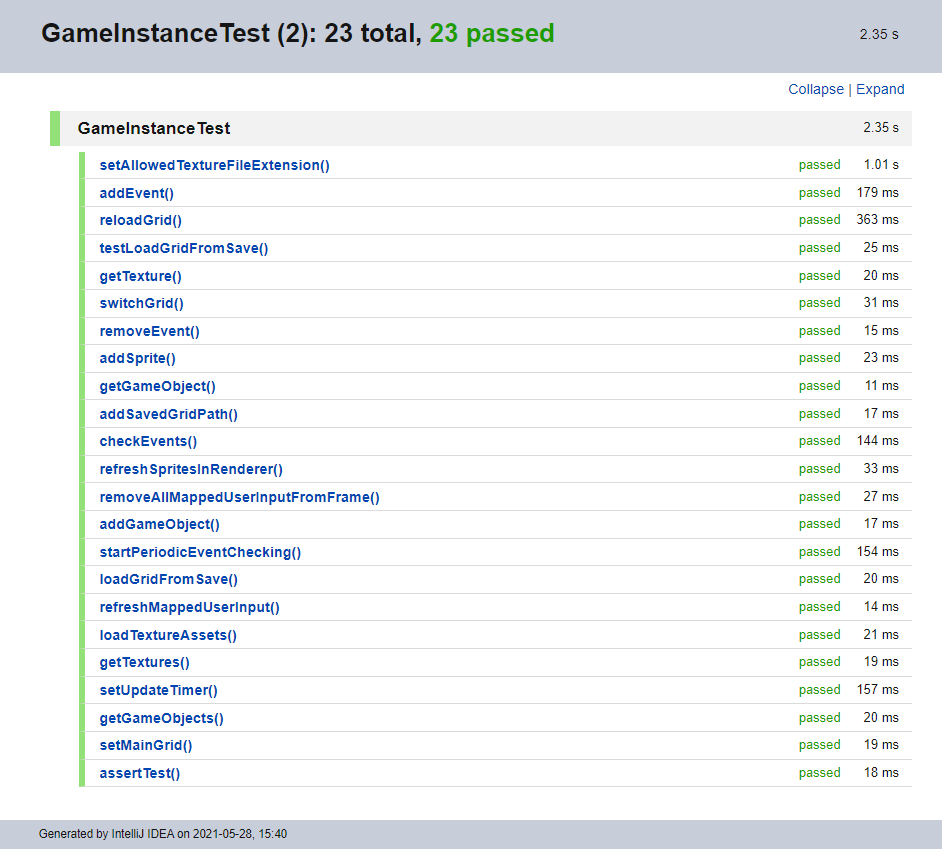
\includegraphics[scale=0.5]{TestRes}
\end{center}

Functional and integration testing was done on the framework but mainly
during the implementation of the two games Sokoban and Sound Board. This
was mainly done by running the map editor and the game on two threads
with the same grid. Doing it this way did for sure generate major issues
(Mainly with swing since they rely on the SwingWorker threads instead of
the standard Java Thread ). In order to somewhat structure these kinds
of tests we utilized the built in debug mode of intellij.

Functional and integration testing can be found in:

\emph{\textasciitilde{}projectRoot} \emph{/Testing/functional/ }

\begin{quote}
\emph{ExtendedMapEditorTest.java}

\emph{BaseFunctionalityTest.java}
\end{quote}

The volume of bugs found this way was massive in comparison to the unit
testing.

Concurrent access

Serialization/deserialization

Visual

Interactions between components

User input issues

Performance issues

Issues relating to excessive swing calls

Using the debug mode in intellij we could generate periodic thread
reports and forcefully cause concurrency issues. After that, find what
threads caused this issue.

One such example is this AWT-EventQueue thread that previously triggered
ConcurrentAccessExceptions:

https://gyazo.com/0c153fbf1078ab255c078941bc941995

\begin{center}
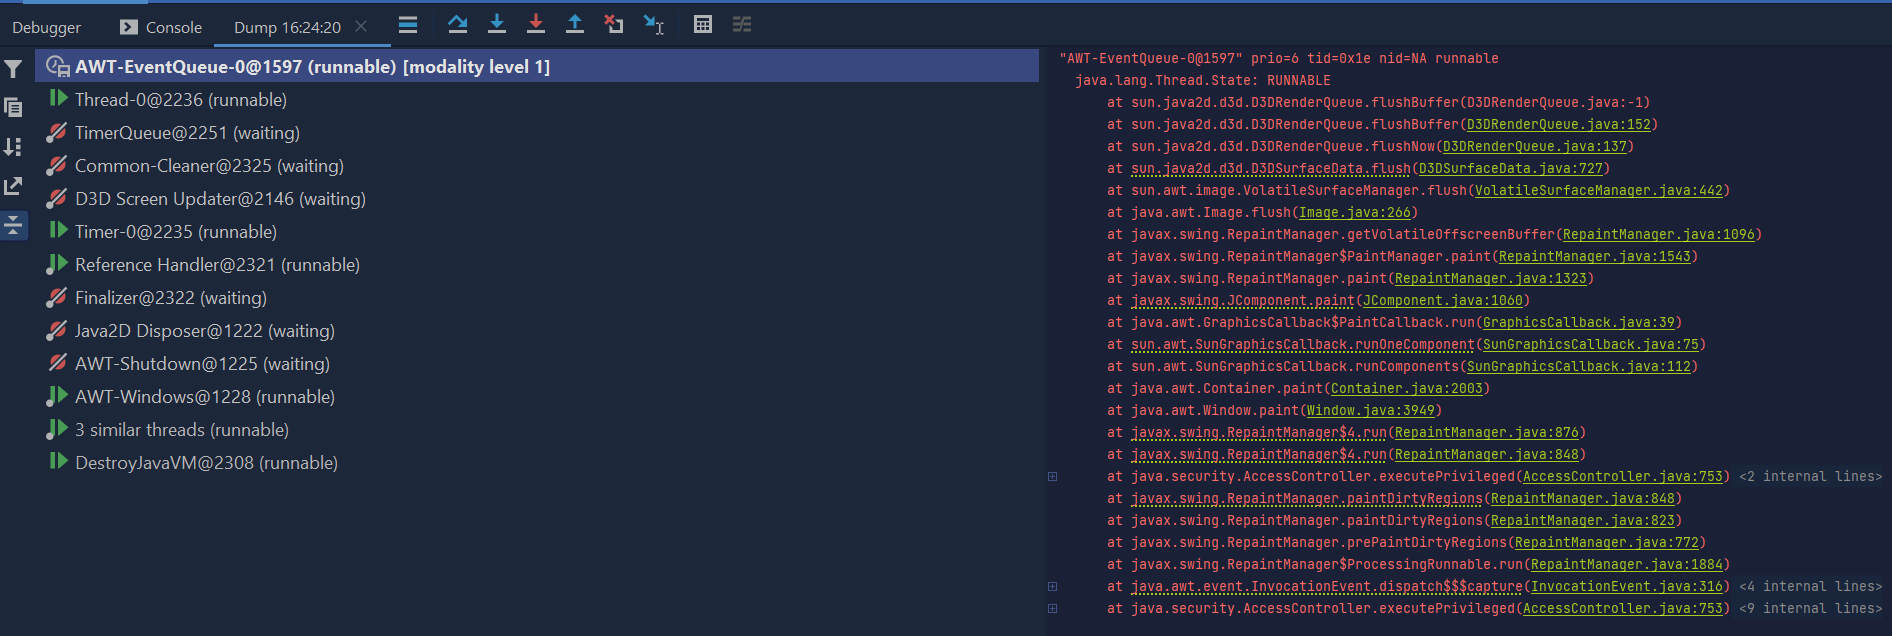
\includegraphics[scale=0.32]{Thread}
\end{center}

Through these reports and github issues displaying similar issues we
managed to find most issues of this sort.

Some issues such as if a thread was stillborn would only be accessible
this way since the read permission is exclusive to the JVM, but since
the intellij debug tools have access to that information through the
frames menu. This was not something that was particularly familiar to us
at first but it uses many of the same concepts that many other IDE's
uses (such as Visual Studio with C\# and IAR EW with C). The level of
access is somewhat hindered since the application runs through the JVM
and not directly on the system.

\end{document}
